\section{Betriebswirtschaftliche Analyse}
\subsection{Beschreibung möglicher Anwendungen aus Business-Sicht}

Auf Basis der bereitgestellten Daten des Online-Shops sollen folgende Fragestellungen beantwortet bzw. Kennzahlen erfasst werden:
\begin{itemize}
 	\item \textbf{Anzahl der Retouren:}\\
 	Es soll die Anzahl der Retouren in Abhängigkeit der Zeit, des Retourengrundes, des Artikels und der Altersgruppe der Kunden analysiert werden. Dabei wird untersucht, ob zum Beispiel bestimmte Artikel besonders häufig wegen eines speziellen Grundes zurückgegeben werden. So könnten Produkte, die besonders häufig aufgrund mangelnder Qualität reklamiert werden, aus dem Angebot entfernt werden. Auch das Alter bzw. das Geschlecht der Kunden könnte aufschlussreiche Informationen zum Reklamationsverhalten liefern und soll daher ebenfalls in diese Analyse einfließen. 
 
 	\item \textbf{Anzahl der Bestellungen:}\\ 
	Auch die Menge der Bestellungen könnte Informationen für geschäftskritische Entscheidungen liefern. Aus diesem Grund soll auch die Anzahl die Bestellungen in Abhängigkeit der Zeit, der Produkte, der Altersgruppen sowie der Herkunft der Kunden betrachtet werden. Mithilfe dieser Analyse lassen sich sowohl die \glqq Top-Seller\grqq ~als auch die \glqq Ladenhütter\grqq ~des Sortiments auf einfache Weise erkennen. Zusammen mit dem Verkaufspreis und der Anzahl der Retouren aus der vorherigen Untersuchung lässt sich so auch die Umsatzverteilung bezogen auf die einzelnen Produkte und Altersgruppen der Kunden berechnen. 
 
 	\item \textbf{Cross-Selling:}\\
 	Mithilfe dieser Analyse soll ermittelt werden, welche Produkte bzw. Produktgruppen besonders häufig zusammen gekauft werden. Auf Basis der Ergebnisse dieser Untersuchung können beispielsweise besondere Angebote oder Produktkombinationen erstellt werden, um so den Umsatz pro Bestellung zu erhöhen.
 	
 	\item \textbf{Einfluss des Newsletters:}\\
 	Da der Online-Shop auch ein Newsletter-Abonnement anbietet, soll auch die Verteilung der Bestellung auf Newsletter-Abonnenten und Kunden ohne Newsletter untersucht werden. 
 
\end{itemize}
 
\pagebreak

\subsection{Konzeptuelle Modellierung}
\subsubsection*{Anzahl der Retouren}

\begin{figure}[htbp] 
  \centering
     \includepdf[pages=2,pagecommand={},scale=1.05,offset=2cm 5.2cm]{phase1/adapt-diagramme.pdf}
\end{figure}

\vspace{11cm}

\subsubsection*{Cross-Selling}
\begin{figure}[htbp] 
  \centering
     \includepdf[pages=4,pagecommand={},scale=1.1,offset=2cm -10.2cm]{phase1/adapt-diagramme.pdf}
\end{figure}

\pagebreak

\subsubsection*{Anzahl der Bestellungen}
\begin{figure}[htbp] 
  \centering
     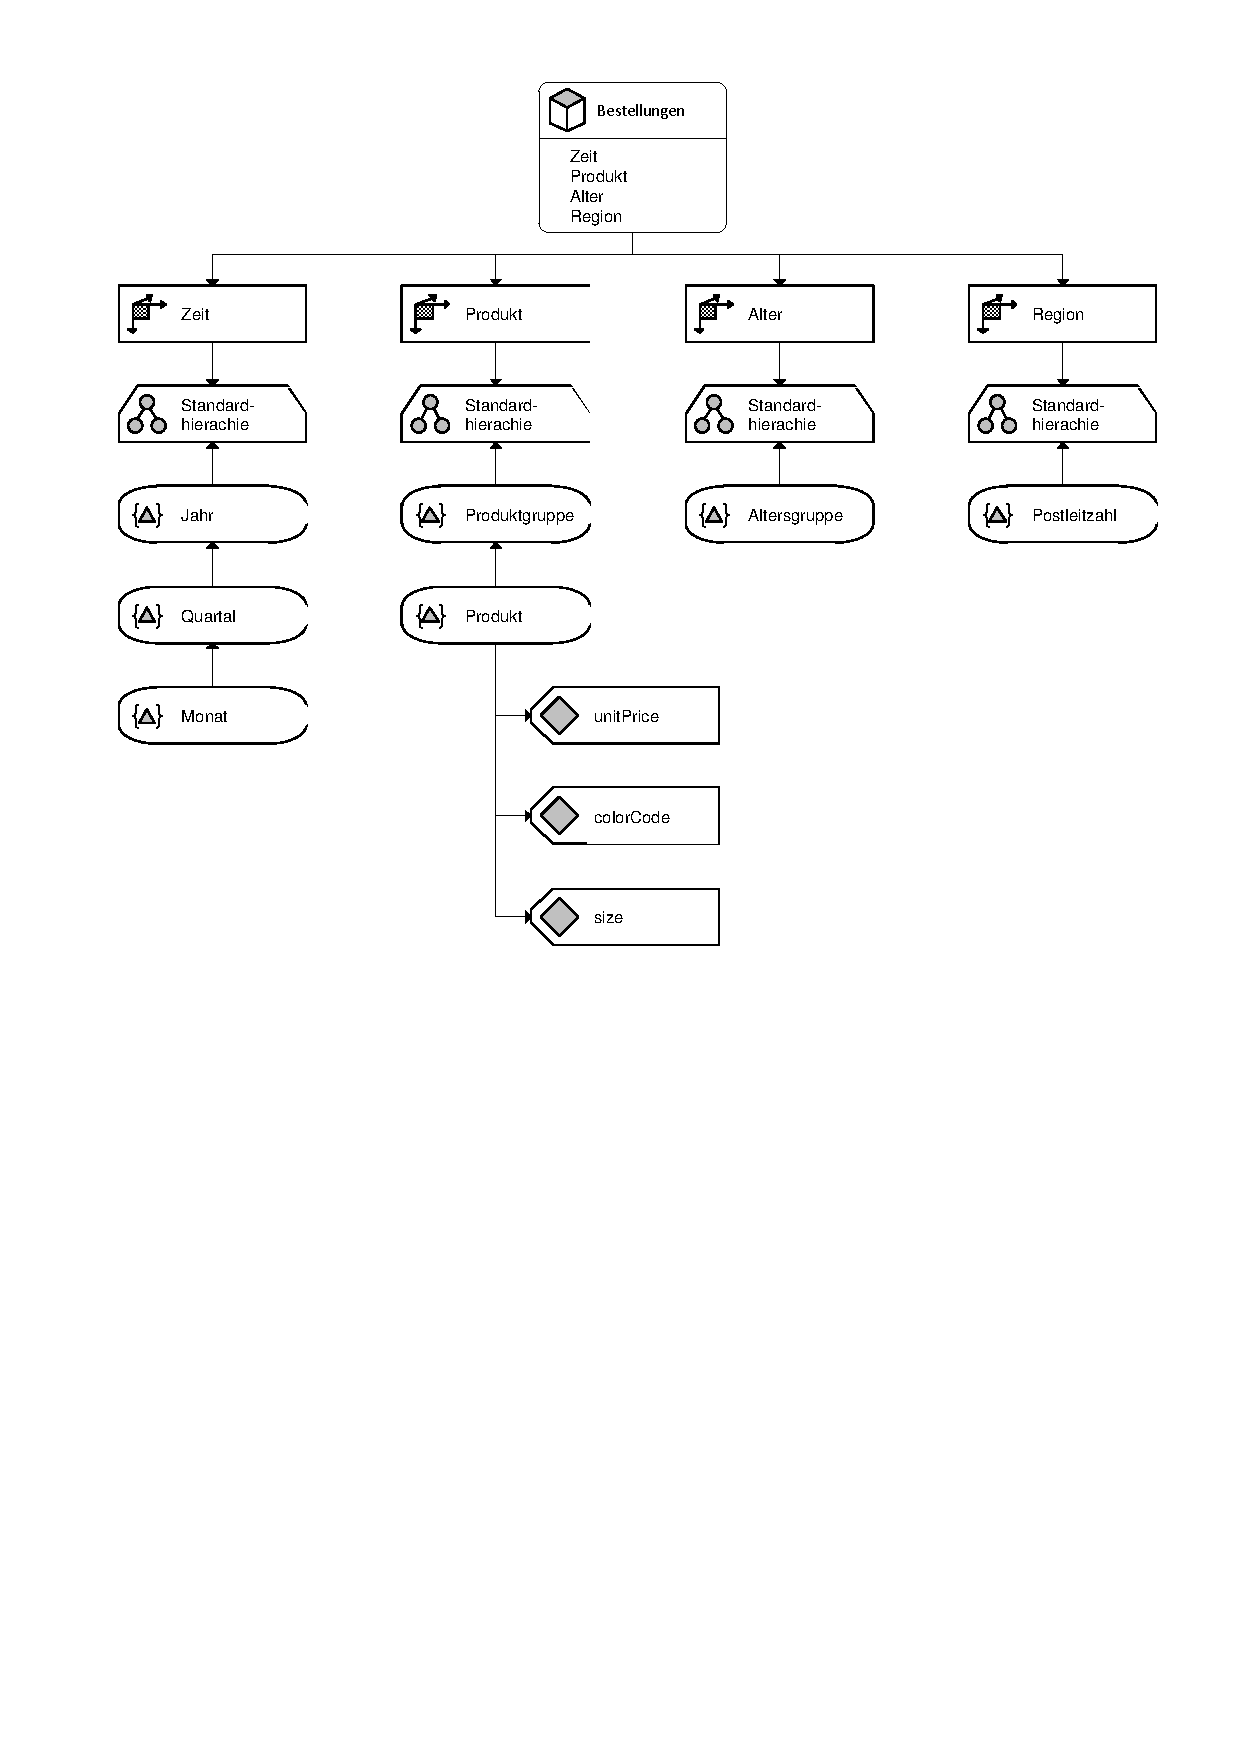
\includepdf[pages=1,pagecommand={},scale=0.8,offset=0cm 0.5cm]{phase1/adapt-diagramme.pdf}
\end{figure}

\vspace{11.6cm}

\subsubsection*{Einfluss des Newsletters}
\begin{figure}[htbp] 
  \centering
     \includepdf[pages=5,pagecommand={},scale=1,offset=0cm -9.3cm]{phase1/adapt-diagramme.pdf}
\end{figure}
\pagebreak

\subsection{Datenverarbeitungsanforderungen}
Da als Datenquelle die operative Datenbank des Online-Shop dient, stellt diese bezogen auf die Granularität, die Aktualität und die Glaubwürdigkeit eine ausreichend hohe Datenqualität bereit.   
Für weiterführende Analysen bezüglich des Gewinns oder der Rentabilität sind die Daten der Datenbank jedoch nicht ausreichend, da Informationen über Einkaufspreise und Ähnliches nicht zur Verfügung stehen. Hierfür müssten externe Datenquellen, wie Preislisten von Großhändlern, in den Analyseprozess integriert werden.

Für das Auslesen der Basisdaten bietet sich eine periodische Extraktion an, da der Fokus bei den Analysen auf der zeitlichen Entwicklung bzw. Verteilung der festgelegten Kennzahlen liegt.
Da in der Dimension \glqq Zeit\grqq ~der Monat die kleinste Konsolidierungsstufe bildet, genügt es die Datenextraktion  ein- bis zweimal im Monat durchzuführen.